\chapter{Les structures}
\label{les-structures}

Dans le chapitre précédent, nous vous avions dit que
les pointeurs étaient entre autres utiles pour manipuler des données
complexes. Les structures sont les premières que nous allons étudier.

Une \textbf{structure} est un regroupement de plusieurs objets, de types
différents ou non. \emph{Grosso modo}, une structure est finalement une
boîte qui regroupe plein de données différentes.

\section{Définition, initialisation et utilisation}
\label{definition,-initialisation-et-utilisation}

\subsection{Définition d'une structure}
\label{definition-dune-structure}

Une structure étant un regroupement d'objets, la première chose à
réaliser est la description de celle-ci (techniquement, sa
\textbf{définition}), c'est-à-dire préciser de quel(s) objet(s) cette
dernière va se composer.

La syntaxe de toute définition est la suivante.

\begin{C}
struct étiquette
{
    /* Objet(s) composant(s) la structure. */
};
\end{C}

Prenons un exemple concret : vous souhaitez demander à l'utilisateur
deux mesures de temps sous la forme
heure(s):minute(s):seconde(s).milliseconde(s) et lui donner la
différence entre les deux en seconde. Vous pourriez utiliser six
variables pour stocker ce que vous fourni l'utilisateur, toutefois cela
reste assez lourd. À la place, nous pourrions représenter chaque mesure
à l'aide d'une structure composée de trois objets : un pour les heures,
un pour les minutes et un pour les secondes.

\begin{C}
struct temps {
    unsigned heures;
    unsigned minutes;
    double secondes;
};
\end{C}

Comme vous le voyez, nous avons donner un nom (plus précisémment, une
\textbf{étiquette}) à notre structure : « temps ». Les règles à
respecter sont les même que pour les noms de variable et de fonction.

Pour le reste, la composition de la structure est décrite à l'aide d'une
suite de déclarations de variable. Ces différentes déclarations
constituent les \textbf{membres} ou \textbf{champs} de la structure.
Notez bien qu'il s'agit de \emph{déclarations} et non de définitions,
l'utilisation d'initialisations est donc exclue.

Enfin, notez la présence d'un point-virgule \emph{obligatoire} à la fin
de la définition de la structure.

\begin{infobox}
Une structure ne peut pas comporter plus de cent vingt-sept membres. 
\end{infobox}


\subsection{Définition d'une variable de type structure}
\label{definition-dune-variable-de-type-structure}

Une fois notre structure décrite, il ne nous reste plus qu'à créer une
variable de ce type. Pour ce faire, la syntaxe est la suivante.

\begin{C}
struct étiquette identificateur;
\end{C}

La méthode est donc la même que pour définir n'importe quelle variable,
si ce n'est que le type de la variable est précisé à l'aide du mot-clé
\mybox{struct} et de l'étiquette de la structure. Avec notre exemple de
la structure \mybox{temps}, cela donne ceci.

\begin{C}
#include <stdio.h>

struct temps {
    unsigned heures;
    unsigned minutes;
    double secondes;
};


int main(void)
{
    struct temps t;

    return 0;
}
\end{C}

\subsection{Initialisation}
\label{initialisation-3}

Comme pour n'importe quelle autre variable, il est possible
d'initialiser une variable de type structure dès sa définition.
Toutefois, à l'inverse des autres, l'initialisation s'effectue à l'aide
d'une liste fournissant une valeur pour chaque membre de la structure.

L'exemple ci-dessous initialise le membre \mybox{heures} à 1,
\mybox{minutes} à 45 et \mybox{secondes} à 30.560.

\begin{C}
struct temps t = { 1, 45, 30.560 };
\end{C}

\begin{attentionbox}
Dans le cas où vous ne fournissez pas
un nombre suffisant de valeurs, les membres oubliés seront initialisés à
zéro ou, s'il s'agit de pointeurs, seront des pointeurs nuls. 
\end{attentionbox}


\subsection{Accès à un membre}
\label{acces-a-un-membre}

L'accès à un membre d'une structure se réalise à l'aide de la variable
de type structure et de l'opérateur \mybox{.} suivi du nom du champ
visé.

\begin{C}
variable.membre
\end{C}

Cette syntaxe peut être utilisée aussi bien pour obtenir la valeur d'un
champ que pour en modifier le contenu. L'exemple suivant effectue donc
la même action que l'initialisation présentée précédemment.

\begin{C}
t.heures = 1;
t.minutes = 45;
t.secondes = 30.560;
\end{C}

\subsection{Exercice}
\label{exercice-5}

Afin d'assimiler tout ceci, voici un petit exercice.\\
Essayez de réaliser ce qui a été décrit plus haut : demandez à
l'utilisateur de vous fournir deux mesures de temps sous la forme
heure(s):minute(s):seconde(s).milliseconde(s) et donnez lui la
différence en seconde entre celles-ci.

Voici un exemple d'utilisation.

\begin{C}
Première mesure (hh:mm:ss.xxx) : 12:45:50.640
Deuxième mesure (hh:mm:ss.xxx) : 13:30:35.480
Il y 2684.840 seconde(s) de différence.
\end{C}

\subsubsection{Correction}
\label{correction-15}

\begin{C}
#include <stdio.h>
#include <stdlib.h>

struct temps {
    unsigned heures;
    unsigned minutes;
    double secondes;
};



int main(void)
{
    struct temps t1;
    struct temps t2;

    printf("Première mesure (hh:mm:ss) : ");

    if (scanf("%u:%u:%lf", &t1.heures, &t1.minutes, &t1.secondes) != 3)
    {
        printf("Mauvaise saisie\n");
        return EXIT_FAILURE;
    }

    printf("Deuxième mesure (hh:mm:ss) : ");

    if (scanf("%u:%u:%lf", &t2.heures, &t2.minutes, &t2.secondes) != 3)
    {
        printf("Mauvaise saisie\n");
        return EXIT_FAILURE;
    }

    t1.minutes += t1.heures * 60;
    t1.secondes += t1.minutes * 60;
    t2.minutes += t2.heures * 60;
    t2.secondes += t2.minutes * 60;

    printf("Il y a %.3f seconde(s) de différence.\n",
    t2.secondes - t1.secondes);
    return 0;
}
\end{C}

\section{Structures et pointeurs}
\label{structures-et-pointeurs}

Certains d'entre vous s'en étaient peut-être doutés : s'il existe un 
objet d'un type, il doit être possible de créer un pointeur vers un
objet de ce type. Si oui, sachez que vous aviez raison. :)

\begin{C}
struct temps *p;
\end{C}

La définition ci-dessus créer un pointeur \mybox{p} vers un objet de
type \mybox{struct\ temps}.

\subsection{Accès via un pointeur}
\label{acces-via-un-pointeur}

L'utilisation d'un pointeur sur structure est un peu plus complexe que
celle d'un pointeur vers un type de base. En effet, il y a deux choses à
gérer : l'accès via le pointeur et l'accès à un membre. Intuitivement,
vous combineriez sans doute les opérateurs \mybox{*} et \mybox{.}
comme ceci.

\begin{C}
*p.heures = 1;
\end{C}

Toutefois, cette syntaxe ne correspond pas à ce que nous voulons car
l'opérateur \mybox{.} s'applique \emph{prioritairement} à l'opérateur
\mybox{*}. Autrement dit, le code ci-dessus accède au champ
\mybox{heures} et tente de lui appliquer l'opérateur d'indirection, ce
qui est incorrect puisque le membre \mybox{heures} est un entier non
signé.

Pour résoudre ce problème, nous devons utiliser des parenthèses afin que
l'opérateur \mybox{.} soit appliqué \emph{après} le déréférencement, ce
qui donne la syntaxe suivante.

\begin{C}
(*p).heures = 1;
\end{C}

Cette écriture étant un peu lourde, le C fourni un autre opérateur qui
combine ces deux opérations : l'opérateur \mybox{-\textgreater{}}.

\begin{C}
p->heures = 1;
\end{C}

Le code suivant initialise donc la structure \mybox{t} via le pointeur
\mybox{p}.

\begin{C}
struct temps t;
struct temps *p = &t;

p->heures = 1;
p->minutes = 45;
p->secondes = 30.560;

\end{C}

\subsection{Adressage}
\label{adressage}

Il est important de préciser que l'opérateur d'adressage peut
s'appliquer aussi bien à une structure qu'à un de ses membres. Ainsi,
dans l'exemple ci-dessous, nous définissons un pointeurs \mybox{p}
pointant sur la structure \mybox{t} et un pointeur \mybox{q} pointant
sur le champ \mybox{heures} de la structure \mybox{t}.

\begin{C}
struct temps t;
struct temps *p = &t;
int *q = &t.heures;
\end{C}

\subsection{Pointeurs sur structures et fonctions}
\label{pointeurs-sur-structures-et-fonctions}

Indiquons enfin que l'utilisation de pointeurs est particulièrement
propice dans le cas du passage de structures à des fonctions. En effet,
rappelez-vous, lorsque vous fournissez un argument lors d'un appel de
fonction, la valeur de celui-ci est affectée au paramètre correspondant.
Cette règle s'applique également aux structures : la valeur de chacun
des membres est copiée une à une. Dès lors, si la structure passée en
argument comporte beaucoup de champs, la copie risque d'être longue.
L'utilisation d'un pointeur évite ce problème puisque seule la valeur du
pointeur (autrement dit, l'adresse vers la structure) sera copiée et non
toute la structure.

\section{Portée et déclarations}
\label{portee-et-declarations}

Dans les exemples précédents, nous avons toujours placés notre
définition de structure en dehors de toute fonction. Cependant, sachez
que celle-ci peut être circonscrite à un bloc de sorte de limiter sa
\textbf{portée}, comme pour les définitions de variables et les
déclarations de variables et fonctions.

Dans l'exemple ci-dessous, la structure \mybox{temps} ne peut être
utilisée que dans le bloc de la fonction \mybox{main()} et les
éventuels sous-blocs qui la composent.

\begin{C}
int main(void)
{
    struct temps {
        unsigned heures;
        unsigned minutes;
        double secondes;
    };

    struct temps t;

    return 0;
}
\end{C}

Notez qu'il est possible de combiner une définition de structure et une
définition de variable. En effet, une définition de structure n'étant
rien d'autre que la définition d'un nouveau type, celle-ci peut être
placée là où est attendu un type dans une définition de variable. Avec
l'exemple précédent, cela donne ceci.

\begin{C}
int main(void)
{
    struct temps {
        unsigned heures;
        unsigned minutes;
        double secondes;
    } t1;
    struct temps t2;

    return 0;
}
\end{C}

Il y a trois définitions dans ce code : celle du type
\mybox{struct\ temps} , celle de la variable \mybox{t1} et celle de la
variable \mybox{t2}. Après sa définition, le type
\mybox{struct\ temps} peut tout à fait être utilisé pour définir
d'autres variables de ce type, ce qui est le cas de \mybox{t2}.

\begin{infobox}
 Notez qu'il est possible de condenser
la définition du type \mybox{struct\ temps} et de la variable
\mybox{t1} sur une seule ligne, comme ceci.
\begin{C}
 struct temps { unsigned heures; unsigned minutes; double secondes; } t1;
\end{C}
\end{infobox}


S'agissant d'une définition de variable, il est également parfaitement
possible de l'initialiser.

\begin{C}
int main(void)
{
    struct temps {
        unsigned heures;
        unsigned minutes;
        double secondes;
    } t1 = { 1, 45, 30.560 };
    struct temps t2;

    return 0;
}
\end{C}

Enfin, précisions que l'étiquette d'une structure peut être omise lors
de sa définition. Néanmoins, cela ne peut avoir lieu que si la
définition de la structure est combinée avec une définition de variable.
C'est assez logique étant donné qu'il ne peut pas être fait référence à
cette définition à l'aide d'une étiquette.

\begin{C}
int main(void)
{
    struct {
        unsigned heures;
        unsigned minutes;
        double secondes;
    } t;

    return 0;
}
\end{C}

\subsection{Déclarations}
\label{declarations}

Jusqu'à présent, nous avons parlé de définitions de structures,
toutefois, comme pour les variables et les fonctions, il existe
également des déclarations de structures. Une déclaration de structure
est en fait une définition sans le corps de la structure.

\begin{C}
struct temps;
\end{C}

Quel est l'intérêt de la chose me direz-vous ? Résoudre deux types de
problèmes : les structures interdépendantes et les structures comportant
un ou des membres qui sont des pointeurs vers elle-même.

\subsection{Les structures interdépendantes}
\label{les-structures-interdependantes}

Deux structures sont interdépendantes lorsque l'une comprend un pointeur
vers l'autre et inversément.

\begin{C}
struct a {
    struct b *p;
};

struct b {
    struct a *p;
};
\end{C}

Voyez-vous le problème ? Si le type \mybox{struct\ b} ne peut être
utilisé qu'après sa définition, alors le code ci-dessus est faux et le
cas de structures interdépendantes est insoluble. Heureusement, il est
possible de \textbf{déclarer} le type \mybox{struct\ b} afin de pouvoir
l'utiliser \emph{avant} sa définition.

\begin{erreurbox}
Une déclaration de structure crée un type dit \textbf{incomplet}
(comme le type \mybox{void}). Dès lors, il ne peut pas être 
utilisé pour définir une variable (puisque les membres qui composent
la structure sont inconnus). Ceci n'est utilisable que pour
définir des pointeurs.
\end{erreurbox}


Le code ci-dessous résoud le « problème » en déclarant le type
\mybox{struct\ b} avant son utilisation.

\begin{C}
struct b;

struct a {
    struct b *p;
};

struct b {
    struct a *p;
};
\end{C}

Nous avons entouré le mot « problème » de guillemets car le premier code
que nous vous avons montré n'en pose en fait aucun et compile sans
sourciller. :-°

En fait, afin d'éviter ce genre d'écritures, le langage C prévoit
l'ajout de \textbf{déclarations implicites}. Ainsi, lorsque le
compilateur recontre un pointeur vers un type de structure qu'il ne
connaît pas, il ajoute implicitement une déclaration de cette structure
juste avant. Ainsi, le premier et le deuxième code sont équivalents si
ce n'est que le premier comporte une déclaration implicite et non une
déclaration explicite.

\subsection{Structure qui pointe sur elle-même}
\label{structure-qui-pointe-sur-elle-meme}

Le deuxième cas où les déclarations de structure s'avèrent nécessaires
est celui d'une structure qui comporte un pointeur vers elle-même.

\begin{C}
struct a {
    struct a *p;
};
\end{C}

De nouveau, si le type \mybox{struct\ a} n'est utilisable qu'après sa
définition, c'est grillé. Toutefois, comme pour l'exemple précédent, le
code est correct, mais pas tout à fait pour les même raisons. Dans ce
cas ci, le type \mybox{struct\ a} est connu car nous sommes en train de
le définir. Techniquement, dès que la définition commence, le type est
déclaré.

\begin{infobox}
Notez que, comme les définitions, les déclarations (implicites ou non)
ont une portée.
\end{infobox}

\section{Un peu de mémoire}
\label{un-peu-de-memoire}

Savez-vous comment sont représentées les structures en
mémoire ?

Les membres d'une structure sont placés les uns après les autres en
mémoire. Par exemple, prenons cette structure.

\begin{C}
 struct exemple
{
    double flottant;
    char lettre;
    unsigned entier;
};
\end{C}

Si nous supposons qu'un \mybox{double} a une taille de huit octets, un
\mybox{char} de un octet, et un \mybox{unsigned\ int} de quatre
octets, voici ce que devrait donner cette structure en mémoire.

\begin{figure}[htbp]
\centering
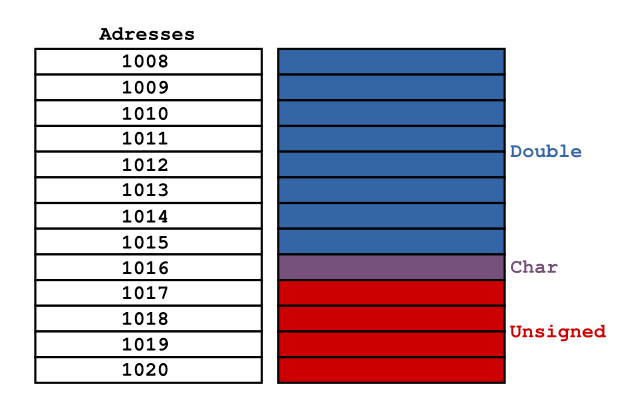
\includegraphics[scale=0.5]{images/structure_memoire.png}
\caption{Représentation en mémoire de la structure}
\end{figure}

\begin{infobox}
Les adresses spécifiées dans le schéma sont fictives et 
ne servent qu'à titre d'illustration.
\end{infobox}


\subsection{L'opérateur sizeof}
\label{loperateur-sizeof}

Voyons à présent comment déterminer cela de manière plus précise, en
commençant par la taille des types. L'opérateur \mybox{sizeof} permet
de connaître la taille en multiplets (\emph{bytes} en anglais) de son
opérande. Cet opérande peut être soit un type (qui doit alors être entre
parenthèses), soit une expression (auquel cas les parenthèses sont
facultatives).

Le résultat de cet opérateur est de type \mybox{size\_t}. Il s'agit
d'un type entier \emph{non signé} défini dans l'en-tête
\mybox{\textless{}stddef.h\textgreater{}} qui est capable de contenir
la taille de n'importe quel objet. L'exemple ci-dessous utilise
l'opérateur \mybox{sizeof} pour obtenir la taille des types de bases.

\begin{C}
#include <stddef.h>
#include <stdio.h>


int main(void)
{
    double f;

    printf("char: %u\n", (unsigned)sizeof(char));
    printf("short: %u\n", (unsigned)sizeof(short));
    printf("int : %u\n", (unsigned)sizeof(int));
    printf("long : %u\n", (unsigned)sizeof(long));
    printf("float : %u\n", (unsigned)sizeof(float));
    printf("double : %u\n", (unsigned)sizeof(double));
    printf("long double : %u\n", (unsigned)sizeof(long double));

    printf("int : %u\n", (unsigned)sizeof 5);
    printf("double : %u\n", (unsigned)sizeof f);
    return 0;
}
\end{C}

\begin{C}
char : 1
short : 2
int : 4
long : 8
float : 4
double : 8
long double : 16
int : 4
double : 8
\end{C}

\begin{infobox}
Le type \mybox{char} a \emph{toujours} une taille de un multiplet.
\end{infobox}


Malheureusement pour nous, la fonction \mybox{printf()} ne fournit pas
d'indicateur de conversion pour le type \mybox{size\_t}\footnote{Depuis
la norme C99, il existe un indicateur de conversion \mybox{zu} qui
permet d'afficher une expression de type \mybox{size\_t}.}. Dès lors,
nous devons recourir à une conversion explicite afin de pouvoir utiliser
un autre indicateur. En l'occurrence, nous avons choisi le type
\mybox{unsigned\ int} étant donné que la taille des types de base est
très petite et qu'il n'y a en conséquence pas de risque de dépasser sa
capacité.

Remarquez que les parenthèses ne sont pas obligatoires dans le cas où
l'opérande de l'opérateur \mybox{sizeof} est une expression (dans notre
exemple : 5 et \mybox{f}).

\begin{infobox}
 Il est parfaitement possible que vous n'obteniez pas les même valeurs que nous,
celles-ci dépendent de votre machine.
\end{infobox}


Ceci étant fait, voyons à présent ce que donne la taille de la structure
présentée plus haut. En toute logique, elle devrait être égale à la
somme des tailles de ses membres, chez nous : 13 (8 + 1 + 4).

\begin{C}
#include <stddef.h>
#include <stdio.h>

struct exemple
{
    double flottant;
    char lettre;
    unsigned int entier;
};


int main(void)
{
    printf("struct exemple : %u\n", (unsigned)sizeof(struct exemple));
    return 0;
}
\end{C}

\begin{C}
struct exemple : 16
\end{C}

\emph{Ah} ! Il semble que nous avons loupé quelque chose\ldots{} :-°

Pourquoi obtenons nous seize et non treize, comme attendu ? Pour
répondre à cette question, nous allons devoir plonger un peu dans les
entrailles de notre machine.

\subsection{Alignement en mémoire}
\label{alignement-en-memoire}

Le processeur et la mémoire vive communiquent entre eux à l'aide d'un
canal appelé un \textbf{bus mémoire}. Les communications à travers le
bus mémoire s'opèrent à l'initiative du processeur qui dispose
d'instructions spécifiques pour déplacer des données de la mémoire vers
un registre et inversement. Ce canal dispose d'une capacité de transport
limitée et ne peut en conséquence transmettre qu'un nombre fixé de
multiplets.

Toutefois, bien que la mémoire vive soit composée de multiplets, le
processeur utilise \emph{toujours} la capacité maximale du bus et lit ou
écrit dans celle-ci par blocs de la taille du bus. Dès lors, le
processeur ne va pas voir la mémoire vive comme une suite de multiplets,
mais comme une suite de blocs de la taille du bus qui sont le plus
souvent appelés des \textbf{mots}.

Quel rapport avec notre structure me direz-vous ? Supposons que notre
processeur lise des blocs de quatre octets à la fois. Si notre structure
faisait treize octets, voici comment le processeur la verrai.

\begin{figure}[htbp]
\centering
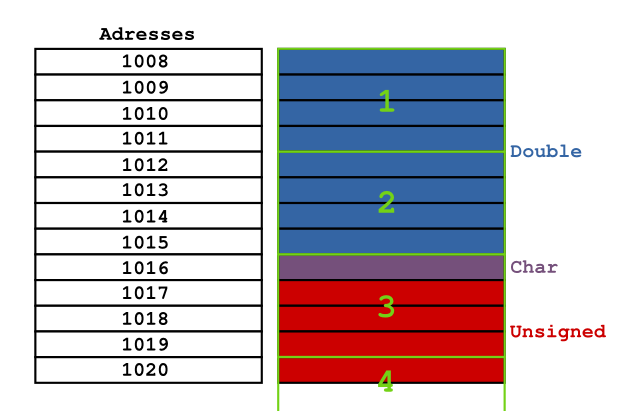
\includegraphics[scale=0.5]{images/vue_memoire_proc.png}
\caption{Vue de la mémoire par le processeur}
\end{figure}

Le premier champ est réparti sur plusieurs mots et remplit complètement
ces mots. Cette situation ne pose pas de problèmes : soit le processeur
charge la donnée en plusieurs fois (ce que la plupart des processeurs
savent faire automatiquement), soit le compilateur prévoit plusieurs
instructions de chargements.

Par contre, le membre de type \mybox{unsigned\ int} est problématique :
vu que sa taille est égale à celle d'un mot, son transfert devrait être
réalisé en une seule fois. Toutefois, dans notre exemple, le membre est
à califourchon sur deux mots. De ce fait, pour obtenir sa valeur, le
processeur devrait :

\begin{itemize}
\item
  charger le troisième mot et en extraire les bons octets ;
\item
  charger le quatrième mot et en extraire le bon octet ;
\item
  et, enfin, combiner le tout pour obtenir la valeur correcte.
\end{itemize}

C'est plus lent, sans compter que quelques rares processeurs ne gèrent
pas ce genre d'opérations et se contentent de signaler une erreur.

\begin{questionbox}
Mais, comment le processeur sait-il que le dernier champ est à cheval sur deux mots ?
\end{questionbox}


À cause de son adresse. Dans notre exemple, le membre de type
\mybox{unsigned\ int} est situé à l'adresse 1017. Étant donné qu'un
\mybox{unsigned\ int} a une taille de quatre octets et que le
processeur lit des mots de quatre octets, il sait que si une donnée de
ce type n'est pas à une adresse multiple de quatre, alors elle est
forcément à califourchon sur deux mots.

Pour éviter ces problèmes, les compilateurs ajoutent des multiplets dit
« de bourrage » (\emph{padding} en anglais), afin d'\textbf{aligner} les
données sur les bonnes adresses. Dans le cas de notre structure, le
compilateur a ajouté trois octets de bourrage juste après le membre de
type \mybox{char} afin que le dernier champ soit forcément à une
adresse multiple de quatre.

\begin{figure}[htbp]
\centering
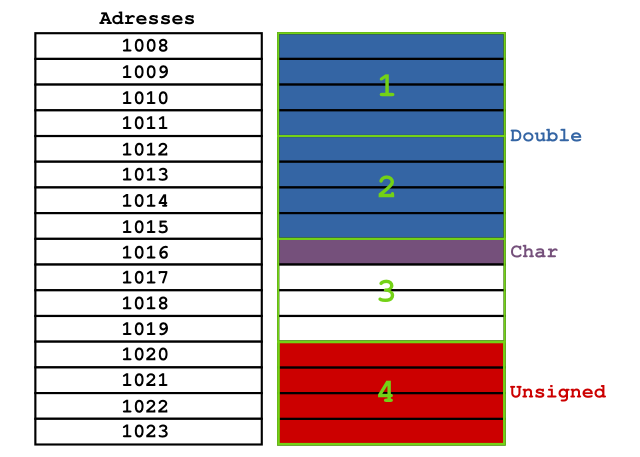
\includegraphics[scale=0.5]{images/structure_correct_align.png}
\caption{La structure correctement alignée}
\end{figure}

\subsection{La macrofonction offsetof}
\label{la-macrofonction-offsetof}

Il vous est possible de connaître les \textbf{contraintes d'alignement}
d'un type (c'est-à-dire le nombre dont doivent être multiple les
adresses d'un type) à l'aide de la \textbf{macrofonction}
\mybox{offsetof()}\footnote{\footnotesize{La norme C11 a introduit un nouvel
  opérateur \mybox{\_Alignof} (et un synonyme \mybox{alignof} fournit
  par l'en-tête \mybox{\textless{}stdalign.h\textgreater{}}) qui donne
  les contraintes d'alignement du type de son opérande. Il s'utilise de
  la même manière que l'opérateur \mybox{sizeof} et retourne lui aussi
  une valeur entière de type \mybox{size\_t}.}} qui est définie dans l'en-tête
\mybox{\textless{}stddef.h\textgreater{}} (nous verrons plus tard ce
qu'est une macrofonction lorsque nous aborderons le préprocesseur).
Cette dernière attends deux arguments : une définition de structure ou
un type de structure et le nom d'un membre de celle-ci. Elle retourne le
nombre de multiplets qui précède ce champ au sein de la structure. Son
retour est de type \mybox{size\_t}, comme pour l'opérateur
\mybox{sizeof}.

Étant donné que le type \mybox{char} prends un multiplet, si le premier
champ d'une structure est de ce type alors le membre suivant sera
forcément précédé du nombre de multiplets de bourrage nécessaire pour
qu'il soit bien aligné. Ainsi, le code suivant vous donne les
contraintes d'alignement pour chaque type de base.

\begin{C}
#include <stddef.h>
#include <stdio.h>


int main(void)
{
    printf("short: %u\n", (unsigned)offsetof(struct { char c; short n; }, n));
    printf("int : %u\n", (unsigned)offsetof(struct { char c; int n; }, n));
    printf("long : %u\n", (unsigned)offsetof(struct { char c; long n; }, n));
    printf("float : %u\n", (unsigned)offsetof(struct { char c; float f; }, f));
    printf("double : %u\n", (unsigned)offsetof(struct { char c; double f; }, f));
    printf("long double : %u\n", (unsigned)offsetof(struct { char c; long double f; }, f));
    return 0;
}
\end{C}

\begin{C}
short: 2
int : 4
long : 8
float : 4
double : 8
long double : 16
\end{C}

\begin{infobox}
Le type \mybox{char} ayant une taille de un multiplet, il peut 
\emph{toujours} être contenu dans un mot. Il n'a donc pas de 
contraintes d'alignement.
\end{infobox}


Pour chaque type, nous définissons une structure composée d'un premier
membre de type \mybox{char} et d'un second membre d'un type dont nous
souhaitons connaître les contraintes d'alignement. Cette définition est
utilisée comme premier argument de la macrofonction \mybox{offsetof()},
le deuxième étant le nom du second membre de la structure. Pour le
reste, le nombre retourné étant de type \mybox{size\_t}, nous opérons à
nouveau une conversion vers le type \mybox{unsigned\ int}.

\hrulefill

Les structures en elles-même ne sont pas compliquées à comprendre, mais 
l'intérêt est   parfois plus difficile à saisir. Ne vous en faîtes pas,
nous aurons bientôt l'occasion de découvrir des cas où les structures se
trouvent être bien pratiques. En attendant, n'hésitez pas à relire le 
chapitre s'il vous reste des points obscurs.

Continuons notre route et découvrons à présent un deuxième type de
données complexes : les \textbf{tableaux}.